\chapterimage{chapters15.png} % Chapter heading image

\chapter{Reiknirit}\index{Reiknitir}\label{k:reiknirit}
\textbf{Reiknirit} (e. algorithm) er forritsbútur sem sinnir sérhæfðum útreikningi.
Dularfyllra er það ekki.
Reiknirit sinna því ákveðnum tilgangi og eru þau oft í grunninn stærðfræðlegs eðlis.

Dæmi um reiknirit sem við höfum séð áður í þessari bók er útfærsla á fjarlægð milli lesta og að setja nýja lestarstöð inn á leið lestar í kóðabút \ref{lst:klasar-aðferðir-lestar}.

Ef nemendur hafa áhuga á að kynna sér tölvunarfræði í framhaldssnámi er gott að hafa fengið nasasjón af því hvað felst í því að beita reikniritum og útfæra þau.
Margir nemendur hefja nám í tölvunarfræði með ýmsar forhugmyndir sem eiga sér sumar ekki stoð í raunveruleikanum.
Þessi kafli og sá næsti fjalla um þau atriði sem leikmenn átta sig ekki endilega á að séu stór hluti af tölvunarfræði og hugbúnaðarþróun; stærðfræði og samvinna.
Þessi kafli er um stærðfræðilegu hliðina og næsti um samvinnuna.

Í þessum kafla ætlum við að skoða nokkur grundvallarreiknirit og hugmyndina um endurkvæmni.

\comment{
\section{Reiknirit sem við höfum séð}\index{Reiknirit sem við höfum séð}\label{uk:reiknirit-okkar}
omg omg omg
\begin{lstlisting}[caption=Við höfum séð eftirfarandi reiknirit, label=lst:reiknirit-okkar]
# kóði
\end{lstlisting}
}

%\section{Þekkt reiknirit}\index{Þekkt reiknirit}\label{uk:reiknirit-þekkt}



\section{Röðun}\index{Röðun}\label{uk:reiknirit-röðun}
Áður en við getum farið að leita ætlum við að raða.
Ímyndum okkur að nokkur spil úr spilastokk séu fyrir framan okkur, þau snúa upp svo við sjáum hvaða spil þetta eru en við sjáum einnig að þau eru ekki í réttri röð.
Sú röð gæti verið hver sem er en gerum ráð fyrir því til einföldunarað þau séu ekki í vaxandi röð með lægsta spilið vinstra megin og hæsta spilið hægra megin.
Hvað er það fyrsta sem við gerum?
Það er ekki eitt svar við því.
Hugsum okkur nú hvert fyrsta skrefið er, svo næsta og koll af kolli.
Reynum svo að lýsa því, eins og með hnetusmjörssamlokuna í kafla \ref{uk:keyra-koda}, þannig að við gætum snúið baki við spilunum (eða bara hvaða spilum sem er sem við höfum ekki séð) og lýst fyrir einhverri annarri manneskju hvernig hún gæti farið að því að raða spilunum með aðferðinni okkar.

Hér er sterklega mælt með því að þið reynið á þessa æfingu áður en lengra er haldið.
Ekki aðeins er hún skemmtileg heldur gætuð þið einnig fundið upp á einhverri nýrri leið til þess að raða.

Ein tiltekin leið til að raða spilunum væri að bera saman fremstu spilin og skipta þeim ef það hærra er vinstra megin og gera það fyrir öll spilin út röðina, skoðum töflu \ref{tbl:insert} til að sjá hvernig það myndi ganga fyrir sig.
Þar erum við með einhverja ákveðna upphafsstöðu á spilunum og byrjum á að skoða fremstu tvö spilin, þá ,,svissum“ við þeim til að hærra spilið sé hægra megin.
Í næstu atrennu ætlum við þá að skoða spilið sem er næst í röðinni og við ,,svissum“ því þangað til það er annað hvort úti í enda eða orðið hærra en það sem er vinstra megin.
Vegna þess að við erum bara með fjögur spil skoðum við þá síðasta spilið og látum það berast niður spilaröðina þar til það passar.


\begin{table}
\begin{center}\begin{tabular}{!{\vrule width 2pt}c!{\vrule width 2pt}P|P|P|P!{\vrule width 2pt}}
	\noalign{\hrule height 2pt}
	\cline{1-5}
	upphafsstaðan &\cellcolor{ocre!30}\textbf{\textcolor{ocre}{K}} & \cellcolor{ocre!30}\textbf{\textcolor{ocre}{10}} & 4 & 8 \tabularnewline
	
	\noalign{\hrule height 2pt}
	& \cellcolor{laurple}10 & \cellcolor{laurple}K & \cellcolor{ocre!30}\textbf{\textcolor{ocre}4} & 8 
	\tabularnewline \hhline{|~|-|-|-|-|}
	
	& \cellcolor{laurple}4 & \cellcolor{laurple}10 & \cellcolor{laurple}K & \cellcolor{ocre!30}¨\textbf{\textcolor{ocre}8} \tabularnewline
	%\cline{1-5}
	%\hline
	\noalign{\hrule height 2pt}
	lokastaðan & \cellcolor{laurple}4 & \cellcolor{laurple}8 & \cellcolor{laurple}10 & \cellcolor{laurple}K \tabularnewline
	\noalign{\hrule height 2pt}
\end{tabular}
\end{center}
\caption{Hér sést hvernig fjórum spilum er raðað í vaxandi röð. Í hverri stöðu er einungis verið að skoða takmarkaðan fjölda spila til að raða, þau spil eru sýnd með grænum lit í töflunni. Þau spil sem búið er að raða eru sýnd með fjólubláum lit.} 
\label{tbl:insert}
\end{table}

Reikniritið sem lýsir þessari röð aðgerða heitir \emph{insertion sort} eða innsetningarröðun og í kóðabút \ref{lst:reiknirit-insertion} ætlum við að skoða hvernig skiptingarnar eiga sér stað.
Á mynd \ref{tbl:insert-abstract} sést hvað er að gerast í einhverju tilteknu skrefi þar sem þarf að finna stað fyrir næsta stak sem á að raða, x.

\begin{table}
	%\begin{table}
		\begin{center}
			\begin{tabular}{c|c |c|c}
				\multicolumn{2}{c}{Búið að raða þessum hluta} &\multicolumn{2}{c}{ Á eftir að raða} \tabularnewline
				\noalign{\hrule height 2pt}
				minna eða jafnt x & stærra en x & x & ??? 
				\tabularnewline \noalign{\hrule height 1.5pt}
				%\tabularnewline
				\multicolumn{4}{c}{\phantom{0}}
				\tabularnewline
				\multicolumn{4}{c}{Í næsta ástandi er röðun orðin:}
				\tabularnewline
				\multicolumn{4}{c}{\phantom{0}}
				
				\tabularnewline
				\multicolumn{3}{c}{Búið að raða þessum hluta} &\multicolumn{1}{c}{ Á eftir að raða}  \tabularnewline
				\noalign{\hrule height 2pt}
				minna eða jafnt x& x & stærra en x  & ??? 
				\tabularnewline \noalign{\hrule height 1.5pt}
			\end{tabular}
		\end{center}
	%\end{table}
\caption{Hér sést í efri línunni hvernig staðan er þegar á að finna stað fyrir eitthvað x, sem gæti verið tala eða spil eða einhver annar hlutur. Athugið að annað hvort eða bæði hólfin, minna eða stærra en x, gætu verið tóm og einnig gæti verið ekkert sem á eftir að raða.
Í neðri línunni sést svo að búið er að finna stað fyrir x á milli staka sem eru lægri en það og staka sem eru hærri en það. Þá myndi þriðja línan vera næsta stak sem er fremst í ??? hlutanum.}
\label{tbl:insert-abstract}
\end{table}



\phantom{easter egg}
%\begin{wrapfigure}{i}{0.2\textwidth} %i o r l 
\begin{center}
	
\includegraphics[scale=1.1]{doodles31-07.png}
\end{center}
%\end{wrapfigure}

Skoðum nú kóðann á bak við þetta reiknirit.

\begin{lstlisting}[caption=Insertion sort reikniritið, label=lst:reiknirit-insertion]
def insertion_sort(A):
	#raðar í vaxandi röð
	i = 1
	while i < len(A):
		j = i
		while j > 0 and A[j-1] > A[j]:
			#skiptum stökunum ef þau eru ekki rétt röðuð
			aj = A[j]
			ajminus = A[j-1]
			A[j] = ajminus
			A[j-1] = aj
			j = j - 1
		i = i + 1
\end{lstlisting}

\vspace{0.3cm}

Nokkrar hugmyndir til að ná upp leikni í notkun á reikniritum eru að:
\begin{itemize}
	\item Reyna að nota reikniritið fyrir einhvern lista af tölum.
	\item Reyna að finna leið til þess að gera línur 8-11 í einni línu, Python býður upp á það.
	\item Reyna að láta reikniritið raða í minnkandi röð.
\end{itemize}

Allar þessar æfingar krefjast þess að við skiljum náið hvað það er sem er að gerast í hverju skrefi og hvers vegna röð skrefanna er eins og hún er.
Markmiðið okkar er að skilja það sem við höfum í höndunum og geta unnið með það á okkar eigin forsendum.

\vspace{0.3cm}

Í kóðabút \ref{lst:reiknirit-bubble} sjáum við útfærslu á \textit{bubble sort}.
Útfærslan felst í tveimur hreiðruðum for-lykkjum.\footnote{Það er yfirleitt ekki góðs viti þegar kemur að tímaflækju, enda er hægt að gera ráð fyrir að tíminn sem það tekur að keyra bubble sort sé $n^2$, sem segir kannski ekkert fyrir óþjálfað auga en hægt er að treysta því að það er ekki ákjósanlegt.}
Reikniritið virkar í grunninn þannig að það tekur við lista sem á að raða.
Það rúllar í gegnum listann frá upphafi og út í enda og ýtir stærsta stakinu út í enda, eins og loftbólur sem þrýstast upp á yfirborðið.


Þegar búið er að rúlla einu sinni í gegnum listann er stærsta stakið komið út í enda og það stak er ekki skoðað aftur heldur álitið á sínum stað.

\begin{wrapfigure}{r}{0.5\textwidth} %i o r l 
	\begin{center}
		
\includegraphics[scale=1.4]{doodles31-25.png}
	\end{center}
\end{wrapfigure}
Þá er aftur rúllað í gegnum listann og stakið sem er þá stærst fer út í enda vinstra megin við stakið sem var stærst.
Þannig að ytri for-lykkjan keyrir fyrir hvert stak í listanum, eða segir til um hversu oft þurfi að finna stærsta stakið, og innri lykkjan sér um samanburðinn og skiptingarnar.
Tökum sérstaklega eftir þar að við getum horft á næsta stak hægra megin þegar við erum að bera saman og það er vegna þess að við hættum fyrir framan aftasta stakið hverju sinni í innri lykkjunni.
%Ef við myndum bara beita breytunni \texttt{vinstri\_hlid} sem \texttt{n-i} þá myndum við fá vísisvillu því við værum að vísa út fyrir listann okkar en vegna þess að við lækkum okkur um 1 þar að auki þá er möguleiki að skoða \texttt{listi[j+1]} sem er næsta stak hægra megin við það stak sem við erum stödd í \texttt{listi[j]}.

\begin{center}
	
\includegraphics[scale=0.8]{doodles31-13.png}
\end{center}
\newpage

\begin{lstlisting}[caption=Bubble sort reikniritið, label=lst:reiknirit-bubble]
	def bubblesort(listi):
	# n er þá fjöldi staka í listanum
	n = len(listi)
	
	# Förum í gegnum öll stökin
	for i in range(n):
		# vinstri hliðin er óröðuð 
		# í fyrstu ítrun er i 0 og vinstri_hlid er því jöfn n-1
		# sem er síðasta stakið í listanum
		# svo verður vinstri_hlid alltaf minni og minni
		# Því síðustu i stökin eru komin á sinn stað
		vinstri_hlid = n-i-1
		
		for j in range(0, vinstri_hlid):
			vinstra = listi[j]
			haegra = listi[j+1]
			# Hér förum við frá 0 upp í n-i-1
			# af því að viljum byrja úti í vinstri enda 
			# og við viljum geta skoðað næsta stak fyrir aftan
			# 
			# Svo skiptum við á stakinu við stakið hægra megin
			# ef stakið er stærra en það sem er hægra megin
			if vinstra > haegra:
			listi[j] = haegra
			listi[j+1] = vinstra
		
	return listi
\end{lstlisting}

Ástæðan fyrir því að taka fyrir bubblesort og insertion sort er að þetta eru aðferðir sem fólk beitir til að raða hlutum í höndunum.
Það byrjar á að færa öftustu hlutina aftast eða bera saman og skipta um staði, þó auðvitað ekki nákvæmlega eins því að fólk og tölvur eru ekki með sömu takmarkanir. 
Tölvuna vantar þessa gífurlegu yfirsýn sem við höfum og okkur skortir hraðann sem hún hefur.
En þessi tvö reiknirit raða nokkurn veginn eins og innsæið okkar segði okkur að fara að því.


\section{Helmingunarleit}\index{Helmingunarleit}\label{uk:reiknirit-helmingunarleit}
Nú þegar við kunnum að raða getum við farið að leita.
Skoðum nú eitthvert þekktasta reiknirit sem til er. 
Það er helmingunarleit að tölu á bili. 
Hugsum okkur að við séum með raðaðan lista af tölum og við viljum finna eina tiltekna tölu. 
Ef við ættum að skoða hverja einustu tölu í listanum til að finna hana tæki það mjög langan tíma.

\begin{wrapfigure}{i}{0.2\textwidth} %i o r l 
\begin{center}
	
\includegraphics[scale=0.9]{doodles31-16.png}
\end{center}
\end{wrapfigure}
Eða allavega fyrir okkur sem manneskjur, en allur tímasparnaður er góður.
Aðgerðin ,,að skoða spil“ kostar einhvern tíma og því færri þannig aðgerðir sem við þurfum að gera því hraðara er reikniritið okkar.\footnote{Tölvunarfræðingar eru mjög uppteknir af því hvað aðgerðir og reikningar taka mikinn tíma.
Þetta er kallað tímaflækja (e. time complexity) og er tölvunarfræðingum mjög hugleikin.
Tímaflækja helmingunarleitar er sérstaklega lág eða $log_2{n}$ vegna þess að reikniritið helmingar alltaf vandamálið (e. problem space).}

Hugmyndin er sú að verið sé að skoða í fyrstu allan listann sem er raðaður (mjög mikilvægt, annars virkar þetta engan veginn) og miðjugildið er skoðað.
Ef gildið sem við leitum að er stærra en miðjugildið eigum við að vera að leita þeim megin við miðjugildið sem stærri gildi eru.
Svo gerum við þetta endurtekið, helmingum alltaf vandamálið þar til við höfum annað hvort fundið gildið sem við leitum að eða þegar bilið sem við erum að leita á inniheldur engin stök.


\begin{lstlisting}[caption=Helmingunarleit að tölu í röðuðum lista með lykkju, label=lst:reiknirit-helm-for]
	def helmingunarleit_med_lykkju(listi, x):
	# Þetta fall tekur við lista sem er raðað í vaxandi röð
	# og gildi sem á að leita að í listanum
	# Þetta er gert með lykkju og án endurkvæmni
	
	# Fallið skilar sætisvísinum sem gildið er í eða -1 ef gildið er ekki í listanum
	
	# minnsti og hæsti vísirinn í listanum
	minnsti = 0
	haesti = len(listi)-1
	
	while minnsti <= haesti:
		# Þetta keyrist á meðan minnsti er enn minni eða jafn og haesti, það er við erum enn með bil til að leita á
	
		midjan = int((minnsti + haesti)/2)
		if listi[midjan] == x:
			# við fundum gildið og skilum vísinum sem það er í
			return midjan
		if listi[midjan] > x:
			haesti = midjan - 1
		else:
			minnsti = midjan + 1
	
	# lykkjan hætti keyrslu svo minnsti vísirinn er orðinn hærri en sá hæsti og þá vitum við að talan er ekki í listanum 
	# við skilum því tölunni -1 til að segja að það hafi ekki verið vísir sem x var í
	return -1
\end{lstlisting}

\section{Endurkvæmni}\index{Endurkvæmni}\label{uk:reiknirit-endurkvæmni}
\textbf{Endurkvæmni} (e. recursion) er sú virkni forrits að vísa í sig sjálft.
Þið þekkið eflaust listaverk sem virka eins og skynvillur, þar sem manneskja getur labbað í hring upp stiga en endað á sama stað því stiginn fer í raun í hring. 
Eða þið hafið séð ykkur sjálf í spegli þar sem var annar spegill fyrir aftan og þið sáuð ótal spegilmyndir raðast af ykkur.
\begin{figure}[h]
	\centering
	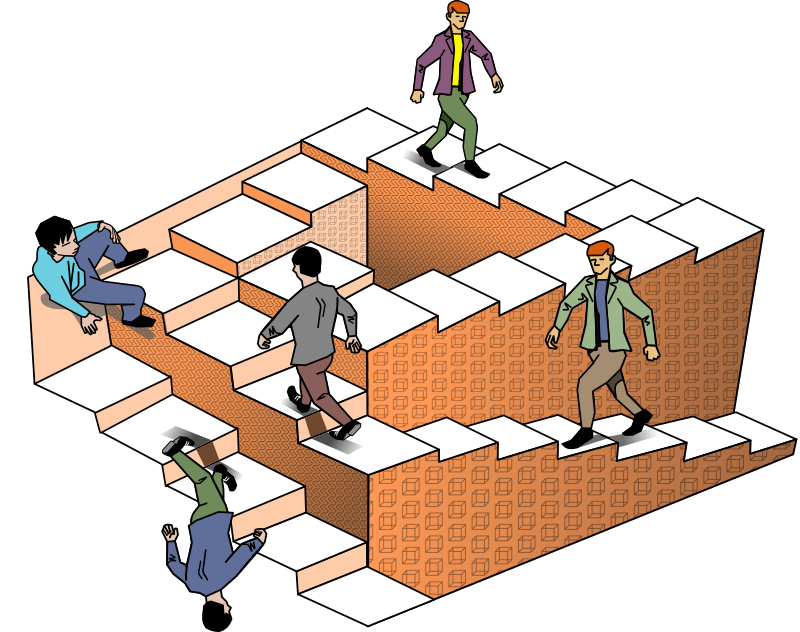
\includegraphics[width=0.50\textwidth]{stairs.png}
	\caption{Mynd í anda Escher fengin af openclipart.org}
	\label{fig: Escher}
\end{figure}

Reynum að átta okkur vel á þessu áður en við reynum að beita því.
Tökum aðeins óhlutbundnara dæmi.
Ímyndum okkur að börn standi í röð og bíði eftir fríum ís, manneskjan sem sér um ísinn snýr sér að fremsta barninu og segir ,,hvað viljiði marga íspinna?“
Barnið vill einn en veit það ekki hvað hin börnin vilja svo það snýr sér að barninu fyrir aftan sig og segir ,,hvað vilt þú marga?“ 
Það barn gerir það sama þangað til þau eru komin út í enda, það barn hefur ekkert annað barn til að spyrja og segir bara ,,tíu íspinna takk“.
Þá veit næstaftasta barnið að það eru allavega 10 íspinnar og svo 2 fyrir það sjálft.
Þannig leggjast tölurnar saman þar til fremsta barnið getur sagt ,,59 íspinna takk fyrir okkur“.


\begin{wrapfigure}{o}{0.35\textwidth} %i o r l 
	\begin{center}
		
\includegraphics[scale=0.9]{doodles31-23.png}
	\end{center}
\end{wrapfigure}
Gott dæmi um hvernig má beita endurkvæmni til að fá skilmerkilega niðurstöðu er að útfæra fall sem reiknar fyrir okkur einhver gildi í Fibonacci röðinni.\footnote{\href{https://en.wikipedia.org/wiki/Fibonacci_number}{Skoðið ensku Wikipediu til að kynnast Fibonacci röðinni}}
Áður en við gerum það skulum við skoða enn einfaldara dæmi þar sem við erum með fall sem kallar í sig sjálft og gerir ekkert annað en það.
Í kóðabút \ref{lst:reiknirit-endurkvæmni1} sjáum við einfalda útgáfu af endurkvæmni, þar sem hugmyndin er í raun kynnt án þess að fallið sé neitt gagnlegt.
Það eina sem fallið gerir er að athuga hvort tala sé stærri en núll og ef hún er það kallar fallið í sig sjálft með gildi sem er einum lægra.
Annars ef talan er ekki stærri en núll prentast ,,við kunnum á endurkvæmni“.
Hveru oft ætli það prentist ef við setjum inn töluna 5?

\begin{lstlisting}[caption=Endurkvæmni - einfalt, label=lst:reiknirit-endurkvæmni1]
def endurkvæmt_fall(tala):
	if(tala > 0):
		# á meðan talan er hærri en 0 köllum við aftur í fallið
		# en við köllum í það af gildi einu lægra
		return endurkvæmt_fall(tala-1)
	else:
		# hér erum við komin niður í 0 og prentum eftirfarandi texta
		print('við kunnum endurkvæmni')
		
endurkvæmt_fall(5)
\end{lstlisting}
\lstset{style=uttak}
\begin{lstlisting}
við kunnum endurkvæmni
\end{lstlisting}
\lstset{style=venjulegt}

Við sjáum í kóðabút \ref{lst:reiknirit-endurkvæmni1} að þó að við höfum kallað í fallið með tölunni 5 fengum við bara einu sinni út strenginn ,,við kunnum endurkvæmni“.
Það er vegna þess að við kölluðum í fallið fyrir 5 og það sem fallið gerir fyrir okkur er að klára endurkvæmnina fyrir það kall.
Það verða ekki til fjögur önnur köll, heldur verður fimm að fjórum sem skilar okkur svo niðurstöðunni fyrir þrjá og svo koll af kolli þar til við erum komin niður í núll og þá hættir reikniritið keyrslu.
Í þessu tilfelli skilar það engu til baka upp fallakallið en klárast engu að síður þarna í línu 8 þegar það kemst þangað.


Það sem þetta reiknirit okkar gerir ekki er að skila einhverri niðurstöðu til baka, en nú skulum við skoða endurkvæmt reiknirit sem skilar summu í kóðabút \ref{lst:reiknirit-endurkvæmni-summa}.
Það reiknar summu af einhverri tölu og öllum jákvæðum tölum sem eru lægri en hún, svo talan 5 gæfi útkomuna 5 + 4 + 3 + 2 + 1 sem er 15.
Endurkvæmnin er því fólgin í því að upphaflega fallakallið með summa(100) skilar okkur 100 + summa(99), sem skilar okkur 100 + 99 + summa(98) og svo koll af kolli þar til talan 1 fæst, og við fáum útreikninginn 100 + 99 + ... + 1 sem skilar okkur 5050.

Einnig skulum við skoða fall sem reiknar n-tu töluna í Fibonacci rununni.
Endurkvæmnin í fib(4) er fólgin í því að skoða alltaf tvær summur í einu en þær skila sér í sama fallakallið.
Þannig skilar fib(4) því sem fib(2) + fib(3) skila.
Kóðann má sjá í kóðabút \ref{lst:reiknirit-endurkvæmni-fib} og á mynd \ref{fig:reiknirit-fib}.
Nú erum við ekki lengur að skila einu gildi og hala af útreikningi heldur erum við að skila tveimur hölum.

\begin{figure}
	\begin{center}
		
		\begin{tikzpicture}[level distance=10mm]
			\tikzstyle{level 1}=[sibling distance=20mm]
			\tikzstyle{level 2}=[sibling distance=10mm]
			\tikzstyle{level 3}=[sibling distance=10mm]
			\node at (0,0) {$f_4$}
			child { node {$f_3$}
				child { node {$f_2$}
					child { node {$f_1$} }
					child { node {$f_0$} }
				}
				child { node {$f_1$} }
			}
			child { node {$f_2$}
				child { node {$f_1$} }
				child { node {$f_0$} }
			};
		\end{tikzpicture}  
	\end{center}
\label{fig:reiknirit-fib}
	\caption{Hér sést hvernig fibonacci fallið kallar alltaf í tvö gildi. Svo eru neðstu gildin, gildin sem vísa ekki í neitt annað, þau sem leggjast saman.}
\end{figure}

\phantom{easter egg}
%\begin{wrapfigure}{i}{0.2\textwidth} %i o r l 
	\begin{center}
		
\includegraphics[scale=0.9]{doodles31-21.png}
	\end{center}
%\end{wrapfigure}


\begin{lstlisting}[caption=Summa reiknuð endurkvæmt, label=lst:reiknirit-endurkvæmni-summa]
def summa(n):
	if n <= 1:
		return 1
	else:
		return n + summa(n-1)

summa(6)
\end{lstlisting}
\lstset{style=uttak}
\begin{lstlisting}
21
\end{lstlisting}
\lstset{style=venjulegt}

\begin{lstlisting}[caption=Fibonacci tölur reiknaðar endurkvæmt, label=lst:reiknirit-endurkvæmni-fib]
def fib(n):
	if n <= 1:
		return n
	else:
		return fib(n-2) + fib(n-1)

fib(4)
\end{lstlisting}
\lstset{style=uttak}
\begin{lstlisting}
3
\end{lstlisting}
\lstset{style=venjulegt}

%\begin{wrapfigure}{i}{0.2\textwidth} %i o r l 
	\begin{center}
		
\includegraphics[scale=1.9]{doodles31-04.png}
	\end{center}
%\end{wrapfigure}

Nú höfum við séð lykkjuútfærslu á helmingunarleit sem keyrir á meðan við höfum bil til að leita á en nú skulum við skoða hvernig má gera þetta endurkvæmt.

\begin{lstlisting}[caption=Helmingunarleit að tölu í röðuðum lista með endurkvæmni, label=lst:reiknirit-helm-end]
def helmingunarleit_med_endurkvaemni(listi, vinstri, haegri, x): 
	# Endurkvæmt fall sem skilar sætisvísinum sem x finnst í í listanum listi
	# Ef x er ekki að finna í listanum listi þá fæst -1
	
	# Athugum hvort að vinstri sé enn vinstra megin
	if haegri >= vinstri: 
	
		# Stillum miðjuna
		midjan = int((vinstri + haegri)/2)
		#midjan = math.floor(vinstri + (haegri - vinstri)/2)
		
		# Athugum hvort gildið sé í miðjustakinu
		if listi[midjan] == x: 
			return midjan 
		
		# Ef gildið er lægra en miðjan þá þurfum við að leita frá vinstri að miðju
		elif listi[midjan] > x: 
			return helmingunarleit_med_endurkvaemni(listi, vinstri, midjan-1, x) 
	
		# Annars hlýtur gildið að vera frá miðju að hægra gildi
		else: 
			return helmingunarleit_med_endurkvaemni(listi, midjan+1, haegri, x) 
	
	else: 
		# Nú er hægra orðið minna en vinstra svo að
		# við erum búin að leita af okkur allan grun
		# gildið er ekki í listanum
		return -1
\end{lstlisting}

%\subsection{Bubble sort}\index{Bubble sort}\label{uk:reiknirit-bubble}
%Nú þegar við höfum leyst það hvernig á að leita að tölu á bili ef bilið er raðað, þá er mikilvægt að skoða hvernig er eiginlega hægt að raða?

%Við höfum séð að listar, innbyggða gagnatagið í Python, hefur innbyggðu aðferðina sort().
%Það sem sort gerði var að breyta lista fyrir okkur þannig að hann væri raðaður í vaxandi röð.

%Nú viljum við hinsvegar átta okkur á því hvernig við getum útfært reiknirit sem raðar fyrir okkur stökum í lista.


%-------------------------------ÆFINGAR----------------------%
\newpage
\section{Æfingar}
\begin{exercise}\label{rei1}
Búið til fall sem tekur við tveimur hnitum, x og y gildum.
Það sem fallið á að gera er að skila tölu sem byggir á því hversu margar hreyfingar hrókur, taflmaðurinn, þyrfti að fara til að komast úr einu hniti í annað.
Í boði eru þrír möguleikar, tvær, ein eða engin hreyfing.

Gerum ráð fyrir að öll möguleg rauntöluhnit séu lögleg fyrir þennan ofurhrók.
\end{exercise}
\setboolean{firstanswerofthechapter}{true}
\begin{Answer}[ref={rei1}]
	\begin{lstlisting}
def hnit(hni11, hnit2):
	# gert er ráð fyrir að hnit sé annað hvort nd eða listi
	if(hnit1 == hnit2):
		return 0
	if(hnit1[0] == hnit2[0] or hnit1[1] == hnit2[1]):
		return 1
	else:
		return 2\end{lstlisting}
\end{Answer}
\setboolean{firstanswerofthechapter}{false}

\begin{exercise}\label{rei2}
Við viljum geta sagt til um hvaða leið er styst og hver er lengst, gefin er ákveðin lestarleið í formi lista af tölum.
Tölurnar tákna hversu langt stoppin eru frá upphafsstöðinni.
Þið eigið annars vegar að búa til fall sem tekur við lista og skilar stystu fjarlægð milli tveggja nærliggjandi stöðva og hins vegar eigið þið að búa til fall sem tekur við sambærilegum lista en skilar lengstu fjarlægð milli tveggja nærliggjandi stöðva.

Athugið að fyrir listann \texttt{[1,3,7,19]} væri svarið 2 fyrir fyrra fallið en 12 fyrir seinna fallið.
Athugið hér sérstaklega bubble sort og hvernig á að skoða tvö stök í einu.
\end{exercise}
\begin{Answer}[ref={rei2}]
Hér er mikið atriði að prófa alls konar mismunandi lista til að vera viss um að þið séuð með kórréttan kóða.
	\begin{lstlisting}
def minnsta_fjarl(listi):
	styst = abs(listi[1]-listi[0])
	for i in range(len(listi)-1):
		if(styst > abs(listi[i+1]-listi[i])):
			styst = abs(listi[i+1]-listi[i])
	return styst

def mest_fjarl(listi):
	mest = abs(listi[1]-listi[0])
	for i in range(len(listi)-1):
		if(mest < abs(listi[i+1]-listi[i])):
			mest = abs(listi[i+1]-listi[i])
	return mest

\end{lstlisting}
\end{Answer}

\begin{exercise}\label{rei3}
Búið til fall sem spyr notandann um fjölda barna sem eru að biðja um íspinna.
Innan þess falls skulið þið vera með fall sem endurkvæmt reiknar út summu íspinna sem börnin vilja.
Notið \texttt{random} kóðasafnið til að búa til einhvern fjölda íspinna sem hvert barn vill.
\end{exercise}
\begin{Answer}[ref={rei3}]
Hér gætum við notað \texttt{input} fallið og \texttt{randint}.
	\begin{lstlisting}
import random as rnd
def ispinnar():
	def summa(fjoldi):
		if fjoldi <= 1:
			return 10
		else:
			return rnd.randint(0,10) + summa(fjoldi - 1)

	fjoldi = input('Hvað eru mörg börn í röðinni? ')
	try:
		int(fjoldi)
		return summa(int(fjoldi))
	except:
		return 10
	\end{lstlisting}
\end{Answer}